\section{Referencia de la Estructura enunciado\-If}
\label{structenunciadoIf}\index{enunciadoIf@{enunciadoIf}}
Clase de almacenamiento de enunciados If en el AST.  


{\tt \#include $<$ast.h$>$}

Diagrama de colaboraci\'{o}n para enunciado\-If:\begin{figure}[H]
\begin{center}
\leavevmode
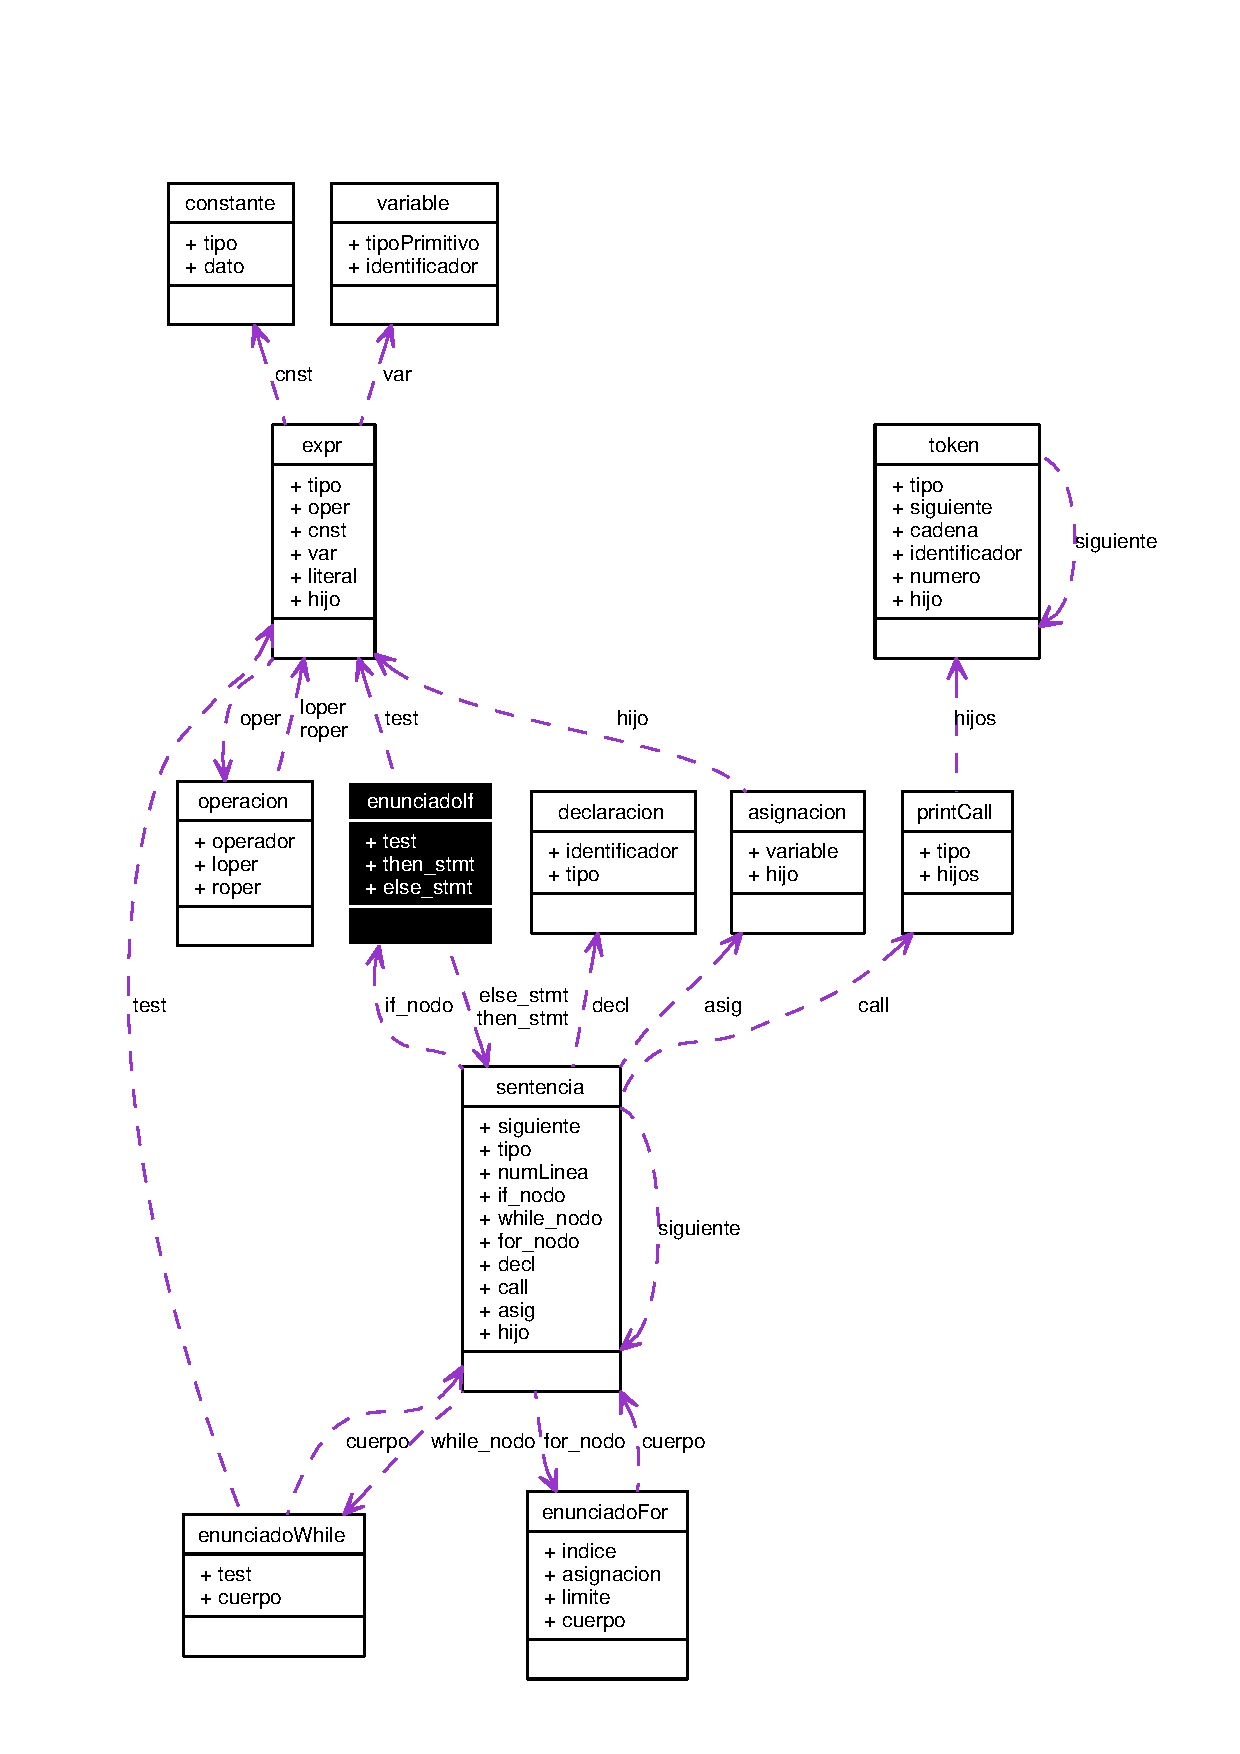
\includegraphics[width=278pt]{structenunciadoIf__coll__graph}
\end{center}
\end{figure}
\subsection*{Atributos p\'{u}blicos}
\begin{CompactItemize}
\item 
{\bf expr} $\ast$ {\bf test}
\begin{CompactList}\small\item\em Expresion booleana a evaluar (if(expr)). \item\end{CompactList}\item 
{\bf sentencia} $\ast$ {\bf then\_\-stmt}
\begin{CompactList}\small\item\em Sentencia o sentencias a evaluar en then. \item\end{CompactList}\item 
{\bf sentencia} $\ast$ {\bf else\_\-stmt}
\begin{CompactList}\small\item\em Sentencia o sentencias a evaluar en else. \item\end{CompactList}\end{CompactItemize}


\subsection{Descripci\'{o}n detallada}
Clase de almacenamiento de enunciados If en el AST. 



Definici\'{o}n en la l\'{\i}nea 186 del archivo ast.h.

\subsection{Documentaci\'{o}n de los datos miembro}
\index{enunciadoIf@{enunciado\-If}!else_stmt@{else\_\-stmt}}
\index{else_stmt@{else\_\-stmt}!enunciadoIf@{enunciado\-If}}
\subsubsection{\setlength{\rightskip}{0pt plus 5cm}{\bf sentencia}$\ast$ {\bf enunciado\-If::else\_\-stmt}}\label{structenunciadoIf_o2}


Sentencia o sentencias a evaluar en else. 



Definici\'{o}n en la l\'{\i}nea 189 del archivo ast.h.

Referenciado por borrar\-If(), evaluar\-If(), y insertar\-Enunciado\-If().\index{enunciadoIf@{enunciado\-If}!test@{test}}
\index{test@{test}!enunciadoIf@{enunciado\-If}}
\subsubsection{\setlength{\rightskip}{0pt plus 5cm}{\bf expr}$\ast$ {\bf enunciado\-If::test}}\label{structenunciadoIf_o0}


Expresion booleana a evaluar (if(expr)). 



Definici\'{o}n en la l\'{\i}nea 187 del archivo ast.h.

Referenciado por borrar\-If(), evaluar\-If(), y insertar\-Enunciado\-If().\index{enunciadoIf@{enunciado\-If}!then_stmt@{then\_\-stmt}}
\index{then_stmt@{then\_\-stmt}!enunciadoIf@{enunciado\-If}}
\subsubsection{\setlength{\rightskip}{0pt plus 5cm}{\bf sentencia}$\ast$ {\bf enunciado\-If::then\_\-stmt}}\label{structenunciadoIf_o1}


Sentencia o sentencias a evaluar en then. 



Definici\'{o}n en la l\'{\i}nea 188 del archivo ast.h.

Referenciado por borrar\-If(), evaluar\-If(), y insertar\-Enunciado\-If().

La documentaci\'{o}n para esta estructura fu\'{e} generada a partir del siguiente archivo:\begin{CompactItemize}
\item 
/media/docs/progra/c++/compiladores1/proy2/godzilla/src/{\bf ast.h}\end{CompactItemize}
